\documentclass{article}

% to avoid loading the natbib package, add option nonatbib:
% \usepackage[nonatbib]{style}

\usepackage[final]{style}

\usepackage[utf8]{inputenc} % allow utf-8 input
\usepackage[T1]{fontenc}    % use 8-bit T1 fonts
\usepackage{hyperref}       % hyperlinks
\usepackage{url}            % simple URL typesetting
\usepackage{booktabs}       % professional-quality tables
\usepackage{amsfonts}       % blackboard math symbols
\usepackage{nicefrac}       % compact symbols for 1/2, etc.
\usepackage{microtype}      % microtypography
\usepackage{amsmath}
\usepackage{verbatim}
\usepackage{graphicx}

\title{Lecture 8: Feature Descriptors and Resizing}

\author{
  \textbf{Harrison Caruthers, Diego Celis, Claire Huang, Curtis Ogren, Junwon Park} \\
  Department of Computer Science\\
  Stanford University\\
  Stanford, CA 94305 \\
  \texttt{\{hdcaruth, dcelis, chuang20, ceogren, junwonpk\}@cs.stanford.edu} \\
}

\begin{document}

\maketitle

\section{Scale invariant keypoint detection}
\subsection{Motivation}
Thus far we have covered detecting keypoints in single images, but broader applications will require such detection across similar images at vastly different scales. For example, we might want to search for pedestrians from the video feed of an autonomous vehicle without prior knowledge of the pedestrians' sizes. Similarly, we might want to stitch a panorama from photos taken at different scales. In both cases, we need to be able to independently detect the same keypoints at those different scales.

\subsection{General methodology}
Currently, we use windows (as in Harris Corner Detection, for example) to detect keypoints. Using the same sized windows will not detect the same keypoints across different sized images (see Figure 1). If we scale the windows appropriately though, they will be able to capturing the same content.

\begin{figure}[h]
  \centering
  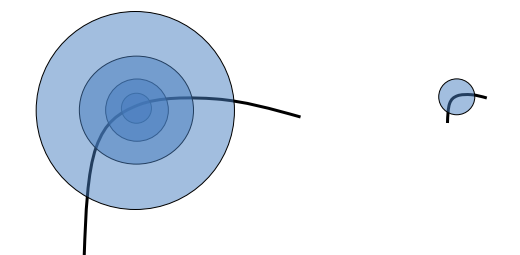
\includegraphics[width=0.55\textwidth]{corners}
  \caption{The corner of a curve appears at two scales. Note that the circular window on the right curve captures the entire corner, while the same-sized window on the left curve does not. Instead, we must choose a much larger circular window on the left curve to get the same information. Source: Lecture 7, slide 12.}
\end{figure}

How do we independently find the correctly scaled windows for each image? We need need to find a way of describing what it means to "capture the same content" in a scale-invariant way. More specifically, consider a function that takes in a region of content and outputs the same value for all scales of that region. Call this function $f(\text{window})$.

Now consider two similar images at different scales. We can independently vary window size for each of the images and plot the response of $f(\text{window})$ as a function of window size:

\begin{figure}[h]
  \centering
  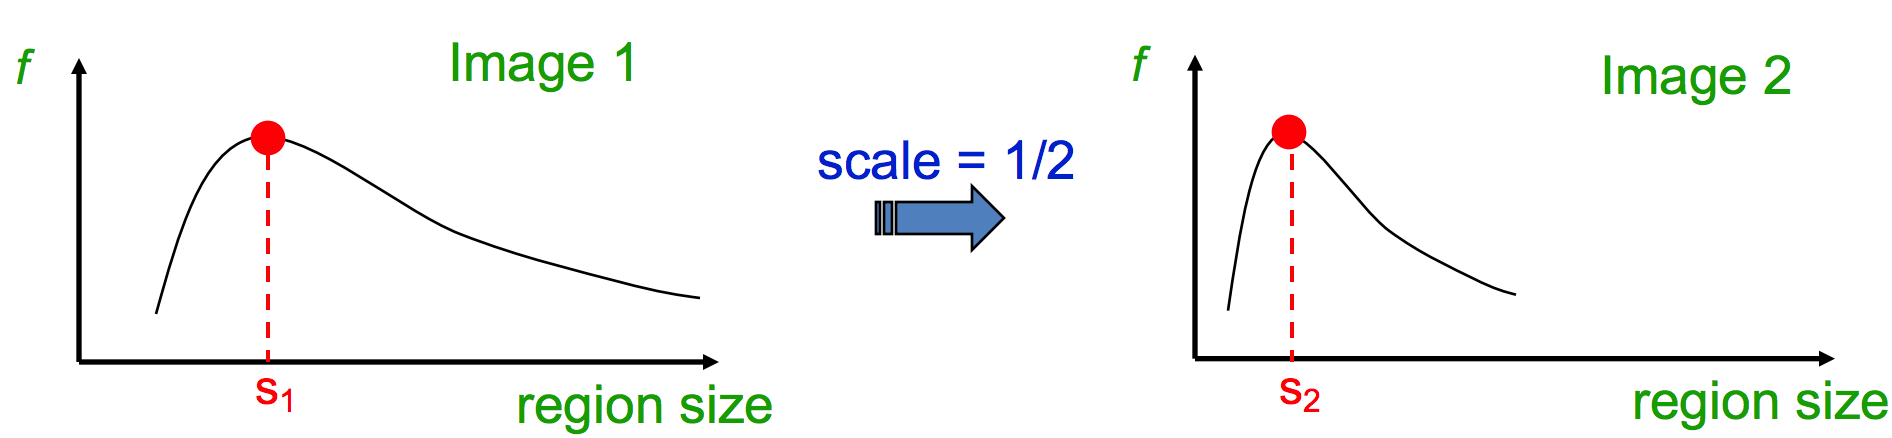
\includegraphics[width=0.75\textwidth]{max}
  \caption{Two plots of the response of $f(\text{window})$ as a function of window size for Images 1 and 2, where Image 2 is similar to Image 1 but scaled by $\frac{1}{2}$. Source: Lecture 7, slide 15.}
\end{figure}

Within each of the two plots, we can independently identify local extrema as keypoints. The window sizes that correspond to those extrema (in the case of Figure 2, $s_1$ and $s_2$) will then tell us the scale difference between the two images.

\subsubsection{Average intensity}
One candidate for such a function $f(\text{window})$ is the average intensity of the pixels within the window, since average intensity doesn't change as we scale the window up or down. 

However, average intensity is not great at capturing contrast or sharp changes within a window, which will make it harder to find clear extrema when comparing $f$ across two images. For capturing contrast, we will need to bring in derivatives into the mix.

\subsubsection{Difference of Gaussians}
Another candidate would be to use the Difference of Gaussians method. 

Consider an image $I$. First, we repeatedly convolve $I$ with Gaussian filters of different $\sigma$'s. Next, we repeat these convolutions with scaled down (i.e. down-sampled) versions of $I$. With this pyramid of Gaussians of different $\sigma$'s and different image sizes (see Figure 3), we then subtract adjacent Gaussian-convolved images to get their difference of Gaussians (DOG):

$$DOG(\sigma) = (G(k\sigma) - G(\sigma)) * I$$

\begin{figure}[h]
  \centering
  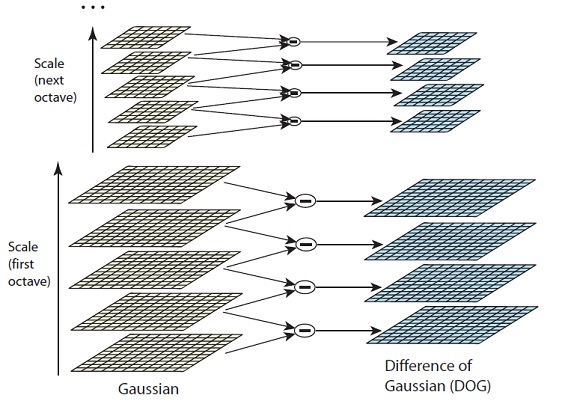
\includegraphics[width=0.45\textwidth]{dog_pyramid}
  \caption{On the left: pyramid of Gaussians of different $\sigma$'s and different image sizes. On the right: difference of adjacent Gaussians. Source: http://aishack.in/tutorials/sift-scale-invariant-feature-transform-log-approximation/}
\end{figure}

Intuitively, these difference of Gaussians capture details about $I$ at different scales. More specifically, the difference of two Gaussians $\sigma_1$ and $\sigma_2$ will remove all details that appear at both $\sigma_1$ and $\sigma_2$ and keep only those details that appear between $\sigma_1$ and $\sigma_2$. The difference of Gaussians for small $\sigma$'s captures fine detail; the difference of Gaussians for large $\sigma$'s captures coarse detail.

Given our differences of Gaussians pyramid in x-y-scale space, we can now identify local extrema within that 3D space to identify both keypoints and their associated scales. To do so, we compare a given coordinate against its 26 neighbors (in 3D space) and deem it an extrema if it is smaller or larger than all neighbors (see Figure 4).

\begin{figure}[h]
  \centering
  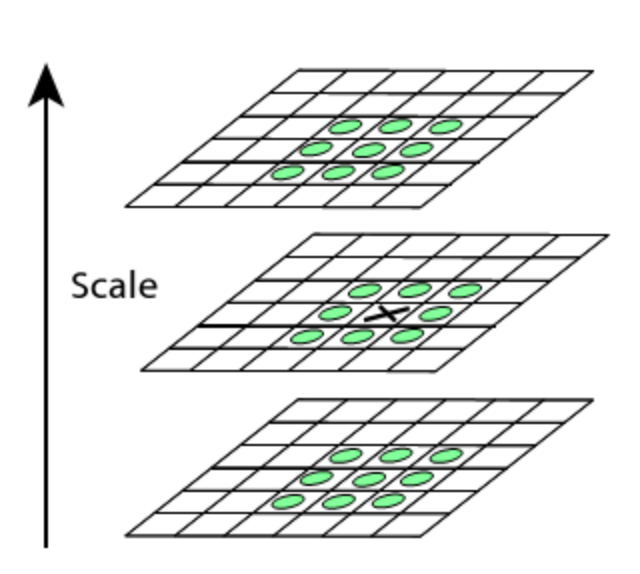
\includegraphics[width=0.3\textwidth]{maxima}
  \caption{Given a coordinate in x-y-scale space (denoted by the black X), examine its 26 neighbors (denoted by the green circles) to determine if the origiinal coordinate is a local extrema. Source: Lecture 7, slide 22}
\end{figure}


\subsubsection{Harris-Laplacian}
A third candidate would be to use the Harris-Laplacian method [2], which has been shown to be more effective at scale-invariant keypoint detection than the difference of Gaussians, but also potentially more computationally expensive.

Consider again an image $I$. First, we create multiple scales of $I$ and run the Harris detector on each to localize keypoints per scale level. We then select the keypoints that maximize the Laplacian across all the scales.

\paragraph{Transition to scale-invariant descriptors:} Now that we have several methods to \textit{detect} consistent keypoints across multiple scales, we can move on to developing methods to \textit{describe} those keypoints in a scale-invariant manner so that they can be matched.

\section{SIFT: an image region descriptor}

\subsection{Invariant Local Features}
Point descriptor should be invariant and distinctive. We transform image content into local feature coordinates that are invariant to translation, rotation, scale, and other imaging parameters to achieve robustness of point descriptors.

Advantages of invariant local features include:
\begin{itemize}
  \item {\bf Locality}: features describe parts, and be robust to occlusion and clutter (no prior segmentation).
  \item {\bf Distinctiveness}: features are identifiable from a large database of objects.
  \item {\bf Quantity}: many features can be generated for even small objects.
  \item {\bf Efficiency}: close to real-time performance.
  \item {\bf Extensibility}: can easily be extended to wide range of differing feature types, each adding robustness to changes.
\end{itemize}

\subsubsection{Scale invariance}
\begin{itemize}
  \item The only reasonable scale-space kernel is a Gaussian. (Koenderink, 1984; Lindeberg, 1994)
  \item An efficient choice is to detect peaks in the difference of Gaussian pyramid (Burt \& Adelson, 1983; Crowley \& Parker, 1984 - but examining more scales)
  \item Difference-of-Gaussian with constant ratio of scales is a close approximation to Lindeberg's scale-normalized Laplacian (can be shown from the heat diffusion equation)
\end{itemize}

\subsubsection{Rotation invariance}
Given a keypoint and its scale from Difference-of-Gaussian(DOG),
\begin{enumerate}
  \item Smooth (blur) the image associated with the keypoint's scale.
  \item Take image gradients over the keypoint neighborhood.
  \item Rotate the gradient directions and locations by negative keypoint orientation. In other words, describe all features relative to the orientation.
\end{enumerate}

\subsubsection{SIFT descriptor formation}
Using precise gradient locations is fragile, so we want to produce a similar descriptor while allowing for generalization. We will create an array of orientation histograms and place gradients into local orientation histograms of 8 orientation bins. Dividing gradients into 8 bins is recommended, and this number of bins was found to exhibit best performance through experimentation. 

More concretely,
\begin{enumerate}
  \item Create array of orientation histograms
  \item Put rotated gradients into local orientation histograms, where each gradient contributes to the nearby histograms based on distance and gradients far from center are scaled down. The SIFT authors authors	found that best results	were with 8 orientations bins per histogram, and a 4x4 histogram array (see Figure 2).
  \item Compare each vector between two images to find matching keypoints.
  \item To add robustness to illumination changes in high contrast photos, normalize the vectors before comparison. Impact from very large image gradients that result from unreliable 3D illumination effects such as glare can be mitigated by clamping values in vector to under 0.2 (an experimentally tuned value) before normalizing again. 
\end{enumerate}

\begin{figure}[h]
  \centering
  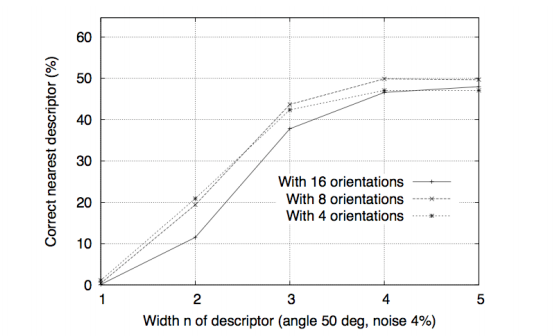
\includegraphics[width=0.75\textwidth]{histogramsensitivity}
  \caption{This figure shows the percentage of correctly matched keypoints as a function of of the width of the descriptor and of the number of histogram bins. [1]}
\end{figure}


\section{HoG: Another image region descriptor}
\subsection{Histogram of Oriented Gradients}
The Hog Descriptor finds an object within an image that pops-out, an object that can be discriminated. The general algorithm for HoG proceeds as follows:
\begin{enumerate}
	\item Divide the image window into small spatial regions or cells. 
    \item For each cell, accumulate a local histogram; group gradient directions into evenly-spaced bins, and allocate the magnitude of a pixel's gradients into the appropriate bin corresponding to the gradient direction  (see Figure 6). 
    \item Normalize the local histograms over a larger region, called a "block" that is comprised of some number of cells.
\end{enumerate}

\begin{figure}[h]
  \centering
  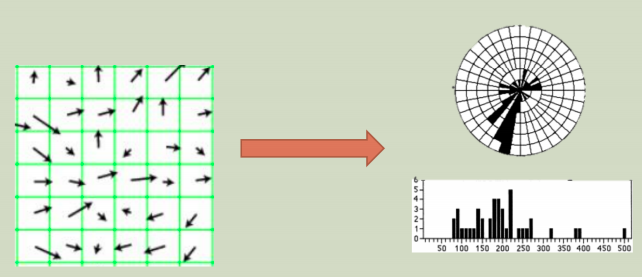
\includegraphics[width=0.75\textwidth]{histogram}
  \caption{Here we see a visual example of keeping track of the magnitudes of the gradients for each gradient direction. Source: Lecture 7, Slide 60.}
\end{figure}

There are a few downsides to using HoG:
\begin{enumerate}
	\item Large variations and ranges when detecting
    \item Very slow
    \item Not very organized when the backgrounds have different illuminations
\end{enumerate}

Despite these downsides, HoG can be quite effective. Note the results of applying HoG in the image below.

\begin{figure}[h]
  \centering
  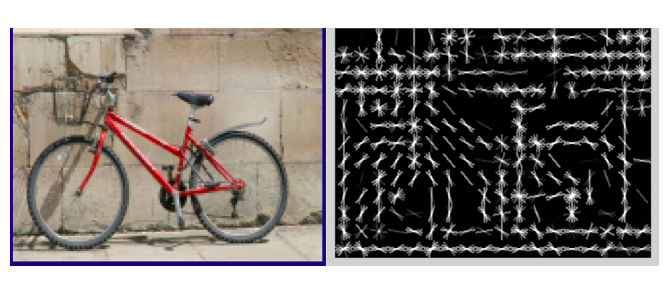
\includegraphics[width=0.75\textwidth]{bike}
  \caption{HoG applied to a bicycle. Source: Lecture 7, Slide 65.}
\end{figure}


\subsection{Difference between HoG and SIFT}
There are some minor differences between the two. HoG is used over an entire image to find gradients. SIFT is used for key point matching.SIFT histograms orient towards the natural positive gradient while HoG does ot. HoG uses neighborhood bins, while SIFT uses weights to compute varying descriptors. 

\section{Image resizing with seam carving}
Because there are different screen sizes, we need to resize content according to display capabilities. Normally, we would try to force content to fill up any kind of display by stretching or shrinking an image. However, this produces less than desirable results. So what's the solution? Content-aware retargeting operators.

\textbf{Retargeting} means that we take an input and ``retarget'' to a different shape or size. Imagine input as being an image of size $n \times m$ and the desired output as an image of size $n' \times m'$. The idea behind retargeting is to
\begin{enumerate}
	\item adhere to geometric constraints (e.g. aspect ratio),
	\item preserve important content and structures, and
	\item limit artifacts.
\end{enumerate}
However, what is considered ``important'' is very subjective, for what may be important to one observer may not be important to another.

\subsection{Pixel energy}

A way to decide what gets to be ``important'' is using \textbf{saliency measures}. There are many different types of saliency measures, but the concept is the same: each pixel $p$ has a certain amount of ``energy'' that can be found by using some function $E$ such that $E(p)$ represents its energy.

The concept is that pixels with higher energy values are more salient, or more important, than pixels with lower energy values. What actually goes into the heart of $E$ is up to the beholder.

A good example is to use the gradient magnitude of pixel $p$ to heavily influence $E(p)$, for this usually indicates an edge. Since humans are particularly receptive to edges, this is a part of the image that is potentially valuable and interesting, compared to something that has a low gradient magnitude. As a result, this preserves strong contours and is overall simple enough to produce nice results. This example of $E$ for image $I$ could be represented as

\begin{align}
	E(\textbf{I}) = \bigg| \frac{\partial \textbf{I}}{\partial x} \bigg| + \bigg| \frac{\partial \textbf{I}}{\partial y} \bigg| \text{.} \nonumber
\end{align}

\subsection{Seam carving}

Let's assume that we have an input image with resolution $m \times n$ and we're looking for an output image $m \times n'$, where $n' < n$. How do we know what pixels to delete? We can use this concept of pixel energy to identify paths of adjacent pixels, or \textbf{seams}, that have the lowest combined pixel energy to remove from the image.

Note that seams need not be strictly rows and columns. In fact, most of the time seams are curves that go through an image horizontally or vertically. A seam is horizontal if it reaches from the bottom edge to the top edge of an image. Similarly, a seam is vertical if it reaches from the left edge to the right edge of an image. However, seams are always laid out in a way such that there is only one pixel per row if the seam is vertical, or only one pixel per column if the seam is horizontal.

In essence, a seam avoids all important parts of an image when choosing what to remove from the image so as to cause the least disruption to the image when removed. There are more things to consider regarding seam carving and use cases that can be improved with similar techniques, but this is the core idea of how seams operate.

\section*{References}
[1] David G. Lowe, "Distinctive image features from scale-invariant keypoints,”  International Journal of Computer Vision, 60, 2 (2004), pp. 91-110

[2] Mikolajczyk, Krystian. “Detection of Local Features Invariant to Affine Transformations.” Perception Group, Institut National Polytechnique de Grenoble, INRIA Grenoble Rhône-Alpes, 2002.


% References
% \small
% \bibliographystyle{plain}
% \bibliography{bibliography}
\end{document}
